\documentclass[14pt,a4paper]{scrartcl}
\usepackage{cmap}
\usepackage[utf8]{inputenc}
\usepackage[T1,T2A]{fontenc}
\usepackage[english,russian]{babel}
\usepackage{relsize}
\usepackage{graphicx}
\usepackage{subfigure}
\usepackage{mathtools}
\usepackage{amssymb}
\usepackage{float}
\usepackage{sidecap}
\usepackage{wrapfig}
\usepackage{caption}
\usepackage[table,xcdraw]{xcolor}
\usepackage{listings}
\usepackage{multirow}
\usepackage{bigstrut}
\begin{document}
	\begin{titlepage}
	\begin{center}
		\large
		МИНИСТЕРСТВО ОБРАЗОВАНИЯ И НАУКИ\\ РОССИЙСКОЙ ФЕДЕРАЦИИ
		
		\vspace{0.5cm}
		
		МГТУ им Н.Э.Баумана
		\vspace{0.25cm}
		
		Факультет ФН
		
		Кафедра вычислительной математики и математической физики
		\vfill
		
		
		Соколов Арсений Андреевич\\
		\vfill
		
		
		{\LARGE Домашнее задание №6 по математической статистике\\[2mm]
		}
		\bigskip
		
		3 курс, группа ФН11-53Б\\
		Вариант 6
	\end{center}
	\vfill
	
	\newlength{\ML}
	\settowidth{\ML}{«\underline{\hspace{0.7cm}}» \underline{\hspace{2cm}}}
	\hfill\begin{minipage}{0.4\textwidth}
		Преподаватель\\
		\underline{\hspace{3cm}} Т.\,В.~Облакова\\
		«\underline{\hspace{0.7cm}}» \underline{\hspace{1.71cm}} 2019 г.
	\end{minipage}%
	\bigskip
	
	
	\vfill
	
	\begin{center}
		Москва, 2019 г.
	\end{center}
\end{titlepage}

\section*{Задание 1}\label{sec1}
В условиях задачи №5 	построить последовательный критерий Вальда для проверки гипотезы $H_0: a=a_0=7.5$  против альтернативы $H_1:a=a_1=8$ при известном $\sigma=\sigma_1=2.5$. Ошибка первого рода $\alpha = 0.1$, ошибка второго рода $\beta = 0.2362404$ вычислена в пункте 4 задачи №5.\\
\textbf{Решение.}\\

Рассмотрим выборку, предложенную нам в условии:
\begin{lstlisting}
> df
[1]  0.653 13.884 11.088  7.409  8.827  5.582  9.747  8.023  8.396
[10]  6.535  6.036  5.251 12.462  9.350  9.770  5.517  6.740 10.759
[19] 10.718  0.840  8.737  2.278  8.447  2.267  8.656  9.460  9.385
[28]  7.924  9.215 10.360  7.239  8.399  7.962  6.712  5.626  7.737
[37]  9.671 13.497 10.708  6.189 10.516  8.845 10.926  8.755  7.728
[46] 12.783  5.300  9.802  5.133  8.534  5.855  5.777 10.128 10.662
[55]  8.307  5.644 10.632  6.060  6.989  5.183  9.587  7.891 15.015
[64]  8.106  9.898 10.504  8.307 10.680  6.788  9.904  6.918  4.250
[73]  8.908  9.837  5.805  6.018  7.735  8.206  5.502  8.473  4.870
[82] 10.159  6.639  7.936  8.149 10.462 12.296  3.403 10.631  7.802
[91]  5.580  8.325 10.687  9.843  9.509  5.668  8.511  8.657  8.835
[100]  9.484
\end{lstlisting}

Критическое множество для среднего при известном среднеквадратическом отклонении запишется в данном случае как $\bar{x} > c_1$, где
\begin{equation*}
c_1 = a_0 + \frac{qnrom(1-\alpha,0,1)}{\sqrt{n}}\sigma_1
\end{equation*}

Имеем:
\begin{lstlisting}
> c1 <- a0 + (qnorm(1-alpha))/(sqrt(df_len)) * sigma1
> c1
[1] 7.820388
\end{lstlisting}

Получаем критическое множество:
\begin{equation*}
	S_1 = \{\bar{x} > 7.820388\}
\end{equation*}

Ошибка второго рода критерия $S_1$ имеет вид:
\begin{equation*}
\beta(c_1) = \Phi(\frac{c_1-a_1}{\sigma_1}\sqrt{n})
\end{equation*}

Имеем:
\begin{lstlisting}
> beta <- pnorm((c1-a1)/sigma1 * sqrt(df_len))
> beta
[1] 0.2362404
\end{lstlisting}

Построим критерий Вальда:
\begin{align*} 
	A = \frac{1-\beta}{\alpha}\\
	B = \frac{\beta}{1-\alpha}
\end{align*}

\begin{lstlisting}
> A <- (1-beta)/alpha
> B <- beta/(1-alpha)
> A
[1] 7.637596
> B
[1] 0.2624894
\end{lstlisting}

\begin{equation*}
	\operatorname{Lf}(\mathrm{j})=\prod_{i=1}^{j} \exp{\left[\frac{z_{i}(a_1-a_0)}{\sigma_1^{2}}+\frac{a_0^{2}-a_1^{2}}{2 \sigma_1^{2}}\right]}
\end{equation*}


Вычислим математическое ожидание момента принятия решения при основной гипотезе $H_0$ и при альтернативе $H_1$.
\begin{align*}
	Y_{k} &=  \ln \frac{p\left(X_{k}, a_1\right)}{p\left(X_{k}, a_0\right)}=\ln \frac{\frac{1}{\sqrt{2 \pi} \sigma}  e^{-\frac{\left(X_{k}-a_1\right)^{2}}{2 \sigma_1^{2}}}}{\frac{1}{\sqrt{2 \pi} \sigma}  e^{-\frac{\left(X_{k}-a_0\right)^{2}}{2 \sigma_1^{2}}}} = -\frac{\left(X_{k}-a_1\right)^{2}}{2 \sigma_1^{2}}+\frac{\left(X_{k}-a_0\right)^{2}}{2 \sigma_1^{2}}=\\
	&= \frac{2 X_{k}(a_1-a_0)+a_0^{2}-a_1^{2}}{2 \sigma_1^{2}}
\end{align*}

\begin{equation*}
	\mathrm{M_0}Y_k=\frac{2 a_0 *(a_1-a_0)+a_0^{2}-a_1^{2}}{2 \sigma_1^{2}}=-\frac{(a_0-a_1)^{2}}{2 \sigma_1^{2}}
\end{equation*}

\begin{lstlisting}
> M0Yk <- -(a1-a0)^2 / (2*sigma1^2)
> M0Yk
[1] -0.02
\end{lstlisting}


\begin{equation*}
\mathrm{M_1}Y_k=\frac{2 a_1 *(a_1-a_0)+a_0^{2}-a_1^{2}}{2 \sigma_1^{2}}=\frac{(a_0-a_1)^{2}}{2 \sigma_1^{2}}
\end{equation*}

\begin{lstlisting}
> M1Yk <- -(a1-a0)^2 / (2*sigma1^2)
> M1Yk
[1] 0.02
\end{lstlisting}

Найдём среднее число испытаний, если верна нулевая гипотеза:
\begin{equation*}
	\mathrm{M_0}\nu = \frac{\alpha \ln(A) + (1-\alpha)\ln(B)}{\mathrm{M_0}Y_k}
\end{equation*}
\begin{lstlisting}
> M0_nu <- (alpha*log(A) + (1-alpha)*log(B))/M0Yk
> M0_nu
[1] 50.0241
\end{lstlisting}

А также среднее число испытаний, если верна альтернативная гипотеза:
\begin{equation*}
\mathrm{M_1}\nu = \frac{\beta \ln(B) + (1-\beta)\ln(A)}{\mathrm{M_1}Y_k}
\end{equation*}
\begin{lstlisting}
> M1_nu <- (beta*log(B) + (1-beta)*log(A))/M1Yk
> M1_nu
[1] 61.84022
\end{lstlisting}

\newpage 

Получили, что при условии $H_0$ потребуется в среднем 50 испытаний, а при условии $H_1$ -- 62 испытания.

\begin{figure}[h]
	\center{\includegraphics[width=1\linewidth]{../img/vald1.png}}
	\label{ris:vald1}
\end{figure}

По графику видим, что кривая пересекает прямую $A$, следовательно, принимаем гипотезу $H_1$.

\newpage

\section*{Задание 2}
Переписать критическое множество из предыдущего пункта в виде $\left(\frac{L\left(\overrightarrow{X_{n}}, a_{1}\right)}{L\left(\overline{X_{n}}, a_{1}\right)} \geqslant C\right)$, отметить на графике и сравнить результаты применения критериев Вальда и Неймана-Пирсона.\\
\textbf{Решение.}\\
Рассмотрим критическое множество критерия Неймана-Пирсона:
\begin{align*}
	S &= \{ \prod\limits_{i=1}^j \exp{\left[\frac{z_{i}(a_1-a_0)}{\sigma_1^{2}}+\frac{a_0^{2}-a_1^{2}}{2 \sigma_1^{2}}\right]} \geqslant C\} = \{ \prod\limits_{i=1}^{100} \frac{z_i(a_1-a_0)}{\sigma_1^2} + 100 \frac{a_0^2-a_1^2}{2\sigma_1^2} \geqslant C_3 \} =\\
	&= \{ \sum\limits_{i=1}^{100} z_i \geqslant C_2 \} = \{ \frac{1}{100}\sum\limits_{i=1}^{100} z_i \geqslant C_1 \},
\end{align*}
где
\begin{align*}
	C_1 &= c_1\\
	C_2 &= 100 \cdot C_1\\
	C_3 &= 100 \frac{a_0^2-a_1^2}{2\sigma_1^2} + C_2 \frac{a_1-a_0}{\sigma_1^2}\\
	C &= e^{C_3}
\end{align*}

\begin{lstlisting}
> C1 <- c1
> C2 <- 100 * C1
> C3 <- 100 * (a0^2-a1^2)/(2*sigma1^2) + C2 * (a1-a0)/(sigma1^2)
> C <- exp(C3)
> C1
[1] 7.820388
> C2
[1] 782.0388
> C3
[1] 0.5631031
> C
[1] 1.756114
\end{lstlisting}

\newpage 
\begin{figure}[h]
	\center{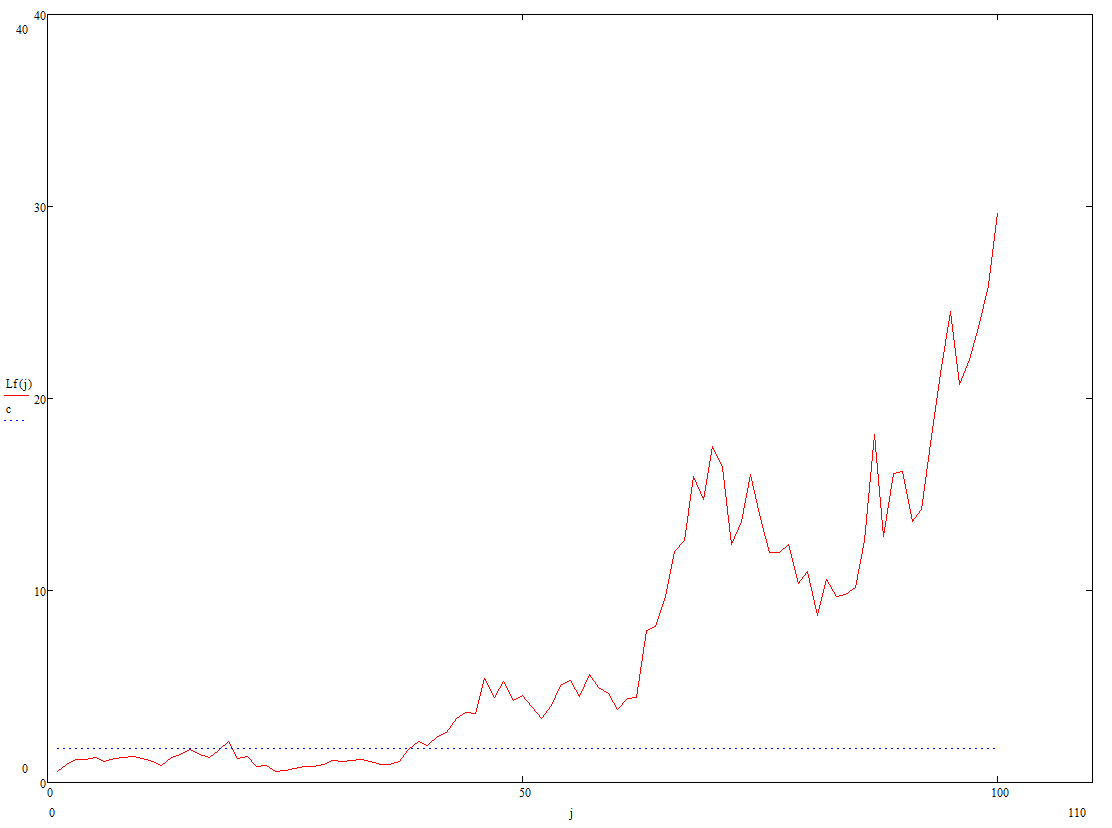
\includegraphics[width=1\linewidth]{../img/neyman-pearson.png}}
	\label{ris:neyman-pearson}
\end{figure}

По графику видим, что кривая на $n=100$ испытании находится над прямой $C$, следовательно принимаем гипотезу $H_1$

Так же можем заметить, что среднее число испытаний в критерии Вальда примерно в два раза меньше, чем для критерия Неймана-Пирсона.



\end{document}